\documentclass[utf8, zavrsni, numeric]{fer}
\usepackage{booktabs}
\usepackage{tabularx}
\usepackage{natbib}
\usepackage{float}

\begin{document}

\nocite{*}

\thesisnumber{5118}

\title{Gusta stereoskopska rekonstrukcija poluglobalnim podudaranjem}

\author{Nikola Bunjevac}

\maketitle

% Ispis stranice s napomenom o umetanju izvornika rada. Uklonite naredbu \izvornik ako želite izbaciti tu stranicu.
\izvornik

% Dodavanje zahvale ili prazne stranice. Ako ne želite dodati zahvalu, naredbu ostavite radi prazne stranice.
\zahvala{}

\tableofcontents

\chapter{Uvod}
Računalni vid iznimno je zanimljivo interdisciplinarno područje koje se svrstava kao grana umjetne inteligencije.
Ono se bavi omogućavanjem računalima da shvate i interpretiraju podatke iz digitalnih slika i videozapisa.
Vid je jedno od najznačajnijih osjetila jer pomoću njega primamo mnoštvo korisnih informacija.
Pomoću vida se orijentiramo u prostoru, prepoznajemo druge ljude i njihova lica, čitamo, prikupljamo informacije itd.
Kada bi računala mogla interpretirati vizualne podražaje poput ljudi, to bi omogućilo velik
napredak u umjetnoj inteligenciji. Nažalost, to je još uvijek neriješen problem.

Cijelo područje
je nastalo šezdesetih godina prošlog stoljeća kada se mislilo da će se taj problem relativno brzo riješiti.
Naime, profesor je kao zadatak studentu zadao da na robota stavi kameru i da robot opisuje ono što vidi.
Vrlo brzo se pokazalo kako je problem puno složeniji nego što se mislilo.
S druge strane, od tada su ostvareni veliki napretci u tom području kao i općenito u umjetnoj inteligenciji.

U ovom radu ćemo opisati neke metode za stvaranje rekonstrukcije prostora iz slika dviju kamera. Takvi sustavi se nazivaju stereo sustavi, a takva vrsta vida stereo vid.
Oni funkcioniraju analogno ljudskom vidu koji se još naziva binokularni vid zbog toga što ljudi gledaju pomoću dva oka. To ljudima omogućava stvaranje vrlo kvalitetnog dojma o 3D osobinama prostora kojeg promatraju. Mogu zaključiti koliko je nešto udaljeno, odnos veličina raznih predmeta itd.

Gusta stereoskopska rekonstrukcija pokušava iz dvaju slika rekonstruirati gusti oblak točaka koji
odgovara prostoru koji se promatra. Postupak se odvija u nekoliko koraka.
Prvo je potrebno obraditi slike kako bi se otklonile fizičke nesavršenosti sustava poput nesavršenosti leće i položaja senzora. Zatim je potrebno piksele
transformirati kako bi svi korespondentni pikseli ležali na istom pravcu, odnosno epipolarnoj liniji. Nakon toga se može krenuti u rekonstrukciju scene.

Postoje dvije glavne podjele metoda guste stereoskopske rekonstrukcije, a to su
\begin{enumerate}
  \item lokalne metode i
  \item globalne metode.
\end{enumerate}

Lokalne metode se temelje na promatranju lokalne okoline svakog pojedinog piksela koju ćemo nazvati prozorčić.
Postupak rekonstrukcije tada se svodi na traženje najsličnijeg prozorčića na drugoj slici. Važno je naglasiti kako se traženje vrši samo duž epipolarne linije.
Za razliku od lokalnih, globalne metode rekonstrukciju rade pomoću svih piksela slike što intuitivno dovodi do zaključka da je postupak složeniji i zahtijeva više računalnih resursa.

Metoda poluglobalnog podudaranja, koju ćemo detaljnije obrađivati u ovom radu, može se svrstati negdje između. Naime, ona kao ulaz prima izračunate korespondencije lokalnih metoda, a zatim radi optimizaciju nad pikselima duž iste linije u osam ili šesnaest smjerova. Takva optimizacije dovodi do kvalitetnijih rezultata u dijelovima gdje dolazi do nagle promjene u dubini scene.

U sljedećem poglavlju ćemo ukratko objasniti postupke kalibracije stereo sustava te rektifikacije parova slika kao predradnja postupku rekonstrukcije.

U trećem poglavlju ćemo obraditi nekoliko lokalnih metoda guste stereoskopske rekonstrukcije. Lokalne metode nude relativno dobre rezultate uz prihvatljivu performansu.

Zatim ćemo definirati algoritam poluglobalnog podudaranja, razraditi njegove hiperparametre te vidjeti kakva poboljšanja nudi u odnosu na lokalne metode.

U petom poglavlju ćemo vidjeti rezultate eksperimenata na standardnim skupovima slika, usporedbe obrađenih metoda i komentare.

U Dodatku A iza zaključka se nalaze kratke upute za korištenje implementiranih programa i skripti za testiranje ispitnih slijedova.

\chapter{Stereoskopska rekonstrukcija}

Prije same rekonstrukcije, potrebno je obraditi slike dobivene iz para kamera. Za to je potrebno znati geometrijske parametre sustava dvaju kamera. Kao model kamere uzet ćemo
projekcijsku ravninu koja je udaljena od izvora/kamere za neku udaljenost $d$. Tako se sve točke u prostoru ispred kamere i ravnine projiciraju na tu zamišljenu ravninu.

\begin{figure}[htb]
  \centering
  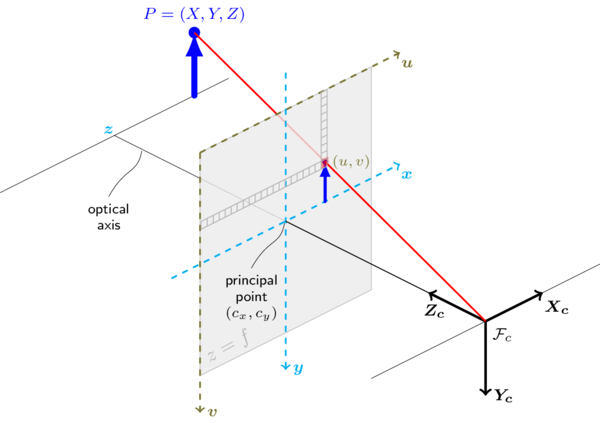
\includegraphics[width=13cm]{img/pinhole_camera_model.png}
  \caption{Model kamere (preuzeto iz dokumentacije biblioteke OpenCV)}
  \label{fig:model-kamere}
\end{figure}


\section{Epipolarna geometrija}

% slika epipolarne geometrije

Geometrijske parametre sustava kamera možemo podijeliti u dvije skupine:
\begin{enumerate}
  \item intrinzični parametri
  \item ekstrinzični parametri.
\end{enumerate}

Intrinzični parametri su svojstveni svakoj kameri pojedinačno, dok su im ekstrinzični parametri zajednički. Neka svojstva koja utječu na intrinzične parametre su nesavršenost leće (radijalna distorzija), pomak senzora
od centra leće (tangencijalna distorzija) i slične fizičke nesavršenosti koje je ponekad nemoguće izbjeći. Stoga priskačemo programskom otklanjanju tih nedostataka.
Ekstrinzični parametri dovode do transformacija kako bismo slike doveli u istu ravninu projekcije te postigli da svi pikseli duž horizontalnog pravca jedne slike odgovaraju istom pravcu (na istoj visini) na drugoj slici. Taj pravac se naziva epipolarna linija. Razlog takvih transformacija je olakšavanje traženja korespondentnih točaka koje sada treba tražiti samo duž epipolarne linije čime je problem sveden na jednu dimenziju. Vidimo da uz malo pretprocesiranja puno olakšavamo problem rekonstrukcije.

\begin{figure}[htb]
  \centering
  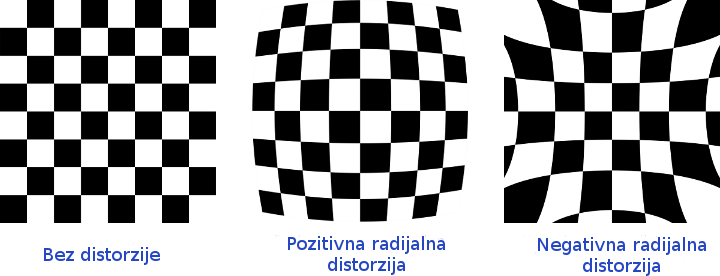
\includegraphics[width=13cm]{img/distortion_examples.png}
  \caption{Primjeri distorzije (preuzeto iz dokumentacije biblioteke OpenCV)}
  \label{fig:primjeri-distorzije}
\end{figure}

\section{Rektifikacija}
Postupak rektifikacije odgovara transformaciji slika kako bismo dobili slike koje zadovoljavaju gore navedena svojstva, a to su:
\begin{enumerate}
  \item Pikseli koji odgovaraju točkama u prostoru na istoj visini nalaze se duž iste epipolarne linije
  \item Nema distorzije uzrokovane lećom
  \item Projekcijske ravnine leže u istoj ravnini
\end{enumerate}
Za rektifikaciju su potrebni ekstrinzični parametri sustava kamera, a za izračun ekstrinzičnih parametara su potrebni intrinzični.
Nakon provedenih transformacija intriznični parametri obaju kamera su jednaki (npr. imaju istu žarišnu udaljenost što je lako predočiti kada znamo da projekcije sada leže u istoj ravnini te je svaka točka
u prostoru ispred jednako udaljena od oba projekcijska platna).

Ovaj postupak se obično provodi uz pomoć šahovske ploče koja je pogodna za to zbog svojih svojstava. Potrebno je parom kamera uslikati dovoljan broj slika na kojima se u potpunosti vidi šahovnica.
Nakon toga se mogu odrediti ranije navedeni parametri. Postupak se odvija u nekoliko koraka, od kojih je prvi traženje šahovskih polja. Nakon toga se pomoću kuteva iz uglova polja može odrediti distorzija
i ostali parametri.

Navedene postupke implementira i nudi biblioteka OpenCV \footnote{http://opencv.org/}. Korisno je istaknuti kako je u korištenim skupovima slika postupak kalibracije i rektifikacije već proveden, barem u skupovima za treniranje. Moguće je doći i do nerektificiranih, sirovih slika pa sam provesti navedene postupke.

% slika epipolarnih linija

\section{Rekonstrukcija udaljenosti}
Sada ćemo opisati postupak za rekonstrukciju udaljenosti pojedinih točaka u prostoru od kamere. Izračun se temelji na određenim disparitetima.

\chapter{Lokalne metode}
Metode guste stereoskopske rekonstrukcije se mogu podijeliti na lokalne i globalne. U ovom poglavlju ćemo načelno opisati takve metode te detaljnije obraditi neke koje su korištene u ovom radu.

Lokalne metode se temelje na principu prozorčića ili okna fiksne širine oko piksela. Označimo širinu prozora s $w$.

Postavlja se pitanje što napraviti na rubovima slike gdje nije moguće izračunati sve vrijednosti. Nekoliko je mogućih rješenja:
\begin{itemize}
  \item računati samo piksele koje je moguće obuhvatiti unutar slike
  \item proširiti sliku crnim okvirom debljine $w/2$
  \item uopće ne računati korespondenciju za rub slike.
\end{itemize}

Svaki pristup ima svoje mane i prednosti. U vlastitoj implementaciji je korišteno treće rješenje gdje se uopće ne računa korespondencija, radi jednostavnosti. Razlika u pogrešci je relativno
mala, a u skupu slika KITTI \footnote{http://www.cvlibs.net/datasets/kitti/eval\_scene\_flow.php?benchmark=stereo} su rubovi uglavnom i isključeni iz provjere točnih dispariteta.

\section{Opći algoritam}
Sada ćemo opisati općeniti algoritam za lokalno podudaranje.

{\tt za svaki piksel $(x, y)$ lijeve slike:}

{\quad \tt za svaki disparitet $0 \leq d \leq maksimalni\_ disparitet$:}

{\quad\quad \tt cijena[$y$][$x$] = $f(x, y, d)$}    


\noindent pri čemu je funkcija $f(x, y, d)$ funkcija korespondencije koja određuje cijenu razlike odgovarajućih piksela lijeve i desne slike. Svaki piksel lijeve slike s pozicijom $(x, y)$
uspoređuje se s pikselom desne slike na poziciji $(x - d, y)$, gdje je $d$ disparitet. Vidimo kako se odgovarajući pikseli nalaze na istoj $y$ koordinati što je posljedica rektifikacije slika.
Stoga je potrebno razmatrati samo piksele duž epipolarne linije.

\section{SSD}

Prva metoda koju ćemo opisati je SSD ({eng. \sl Sum of Squared Differences}) koja se temelji na zbroju kvadrata razlika intenziteta piksela.
Matematički ju možemo opisati sljedećim izrazom:
$$C_{SSD}(x, y, d) = \sum_{i}(I_R(x - d, y) - I_L(x, y))^2 $$
gdje su $(x, y)$ koordinate piksela lijeve slike, $d$ trenutni disparitet, a $I_L$ lijeva slika te $I_R$ desna slika. Zbroj ide po svim pikselima unutar prozora promatranog piksela.
Najbolja podudarnost kod SSD-a postiže se kada je vrijednost funkcije cijene jednaka $0$. Lako je vidjeti zašto je tomu tako kada bismo usporedili dva prozora s istim intenzitetima piksela. Tada će vrijednost funkcije biti $0$ jer oduzimamo iste vrijednosti. Iz toga slijedi da što se intenziteti više razlikuju, to će i cijene biti veće. Također, kvadrat doprinosi tome da vrijednosti ne budu negativne tako da možemo raditi samo s pozitivnim brojevima.

\section{ZSAD}

Sljedeća metoda je ZSAD ({eng. \sl Zero Sum of Absolute Differences}). Matematički ju možemo definirati ovako:
$$C_{ZSAD}(x, y, d) = \sum_{i}\lvert(M_L - I_L(x, y)) - (M_R - I_R(x - d, y))\rvert$$
gdje je $I_L$ lijeva slika, $I_R$ desna slika, a $M_L$ i $M_R$ srednje vrijednosti intenziteta piksela u trenutnom prozoru lijeve, odnosno desne slike.
\section{Census}

Funkcija korespondencije Census se temelji na Hammingovoj udaljenosti između dvije binarne riječi. Kako bismo odredili cijenu između dvaju piksela, potrebno je transformirati
prozore oko piksela u binarne riječi. Svakom pikselu u prozoru ćemo pridružiti bit prema sljedećoj funkciji:

\[   
b(p, q) = 
     \begin{cases}
       0, & I(p) \leq I(q) \\
       1, & I(p) > I(q) \\
     \end{cases}
\]
gdje je $I$ slika, $p$ piksel u sredini prozora za kojega računamo transformaciju, $q$ bilo koji piksel unutar prozora. Važno je napomenuti da redoslijed pridruživanja bitova mora biti jednak u oba
prozora koja se uspoređuju kako bi rezultat bio ispravan. Nakon što svakom pikselu pridružimo binarnu vrijednost, cijenu možemo izračunati
računski tako primijenimo operaciju isključivo-ili između binarnih riječi prozora lijeve i desne slike te zatim prebrojimo broj bitova u jedinici.

\section{Korespondencija neovisna o uzorkovanju}

Birchfield-Tomasijeva korespondencija se malo razlikuje od do sada navedenih metoda. Razlikuje se po tome što ona ne koristi prozorčić već se temelji na usporedbama s dvaju susjednih piksela duž epipolarne linije.
Funkcija cijene je definirana preko simetričnih funkcija:
$$ C_{BT} = min(C_{BT}(x_i, y_i, I_L, I_R), C_{BT}(y_i, x_i I_R, I_L) $$
gdje se $x_i$ i $y_i$ pikseli lijeve slike $I_L$, odnosno desne slike $I_R$.

Funkcije $C_{BT}$ je definirana ovako:
\begin{equation}
I^+ = \frac{1}{2}(I_i(y_i) + I_R(y_i + 1))
\end{equation}

\begin{equation}
I^- = \frac{1}{2}(I_R(y_i) + I_R(y_i - 1))
\end{equation}

\begin{equation}
I_{min} = min(I^-_R, I^+_R, I_R(y_i))
\end{equation}

\begin{equation}
I_{max} = max(I^-_R, I^+_R, I_R(y_i))
\end{equation}

\begin{equation}
C_{BT}(x_i, y_i, I_L, I_R) = max(0, I_L(x_i) - I_{max}, I_{min} - I_L(x_i)))
\end{equation}

Birchfield-Tomasijeva cijena je opisana u diplomskom radu Dine Kovača \citet{kovac15ms}, a izvorno u ...

\section{Usporedba lokalnih i globalnih metoda}
U ovom odjeljku dana je usporedba lokalnih i globalnih metoda podudaranja.
U tablici se nalaze neka važnija svojstva lokalnih metoda s lijeve strane te
analognih svojstava globalnih metoda s desne strane.

\begin{table}[H]
  \caption{Svojstva lokalnih i globalnih metoda}
  \label{tbl:usp_lok_glob}
  \centering
  \begin{tabularx}{\textwidth}{X|X} \hline
    {\bf Lokalne metode} & {\bf Globalne metode} \\
    \hline
    cijene temeljene na prozorčićima oko svakog pojedinog piksela & cijene temeljene na svim pikselima slike \\
    \hline
    odabir pojedinog dispariteta po principu minimalne agregirane cijene & minimizacija globalne funkcije kroz vrijednosti svih piksela slike \\
    \hline
    značajno jednostavnije za implementaciju & teže za implementaciju \\
    \hline
    daju lošije rezultate & daju značajno bolje rezultate \\
    \hline
    u pravilu brže & u pravilu sporije \\
  \end{tabularx}
\end{table}

U sljedećem poglavlju ćemo uvesti algoritam poluglobalnog podudaranja koji kao ulaz prima cijene izračunate kod lokalne korespondencije, a optimizaciju radi nad svim
pikselima u određenim smjerovima. Time ga, kao što mu i naziv govori, možemo svrstati negdje između jer koristi lokalne korespondencije, a optimira (točnije, aproksimira) globalno.


\chapter{Poluglobalno podudaranje}

\chapter{Rezultati}

\begin{figure}[htb]
  \centering
  \includegraphics[width=13cm]{img/SSD.png}
  \caption{Pogreška metode korespondencije SSD}
  \label{fig:SSD-error}
\end{figure}

\begin{figure}[htb]
  \centering
  \includegraphics[width=13cm]{img/ZSAD.png}
  \caption{Pogreška metode korespondencije ZSAD}
  \label{fig:ZSAD-error}
\end{figure}

\begin{figure}[htb]
  \centering
  \includegraphics[width=13cm]{img/Census.png}
  \caption{Pogreška metode korespondencije Census}
  \label{fig:Census-error}
\end{figure}

\chapter{Zaključak}
Zaključak.

\bibliography{literatura}
\bibliographystyle{fer}

\appendix
\chapter{Upute za korištenje}
Ovdje idu upute.

\begin{sazetak}
  Sažetak na hrvatskom jeziku.

\kljucnerijeci{računalni vid, stereoskopska rekonstrukcija, poluglobalno podudaranje, disparitet, korespondencija}
\end{sazetak}

% TODO: Navedite naslov na engleskom jeziku.
\engtitle{Dense stereoscopic reconstruction with semi-global matching}
\begin{abstract}
Abstract.

\keywords{computer vision, stereoscopic reconstruction, semi-global matching, disparity, correspondence}
\end{abstract}

\end{document}
